\documentclass{article}
\usepackage[a4paper, left=3cm, right=2cm, top=3cm, bottom=2cm]{geometry}
\usepackage{graphicx}
\usepackage{amsmath}
\usepackage[shortlabels]{enumitem}
\usepackage{array}
\usepackage{xcolor}
\usepackage{amssymb}
\usepackage{amsthm}
\usepackage{mathtools}
\usepackage{tikz}
\usepackage{pgfplots}
\usepackage{arydshln}
\usepackage{float}
\usepackage{listings}
\usepackage{xcolor}


\pgfplotsset{compat=1.18} % Set pgfplots compatibility level

\lstset{
    language=Python,
    basicstyle=\ttfamily\small,
    keywordstyle=\color{blue},
    stringstyle=\color{red},
    commentstyle=\color{green},
    morecomment=[s][\color{magenta}]{"""}{"""},
    numbers=left,
    numberstyle=\tiny\color{gray},
    stepnumber=1,
    numbersep=10pt,
    showspaces=false,
    showstringspaces=false,
    showtabs=false,
    frame=single,
    tabsize=4,
    captionpos=b,
    breaklines=true,
    breakatwhitespace=false,
    escapeinside={\%*}{*)}
}

\title{
    \textbf{Universidade de São Paulo\\ Escola Politécnica}\\
    \vspace{20pt}
    
\includegraphics[scale=0.5]{images/logo-poli.png} \\
    \vspace{20pt}
    \textbf{PNV5761 - Programação Matemática Aplicada a Problemas de Transporte} \\
    \vspace{10pt}
    \textbf{Quarta série de problemas.}\\
    \vspace{15pt}
    \large{Prof. Marco Antonio Brinati} \\
    \vspace{45pt}
    % \large{Guilherme Fernandes Alves - 10774361} \\
    \vspace{10pt}
    \date{\textbf{\Large{São Paulo, Setembro de 2024}}}
}

\author{Guilherme Fernandes Alves - 10774361}

\begin{document}

\renewcommand{\arraystretch}{1.5}

\maketitle
\newpage

\section{Questão 1}

Considere o problema de transbordo cujo grafo orientado, com os respectivos parâmetros, é mostrado na figura abaixo.

\begin{figure}[H]
    \centering
    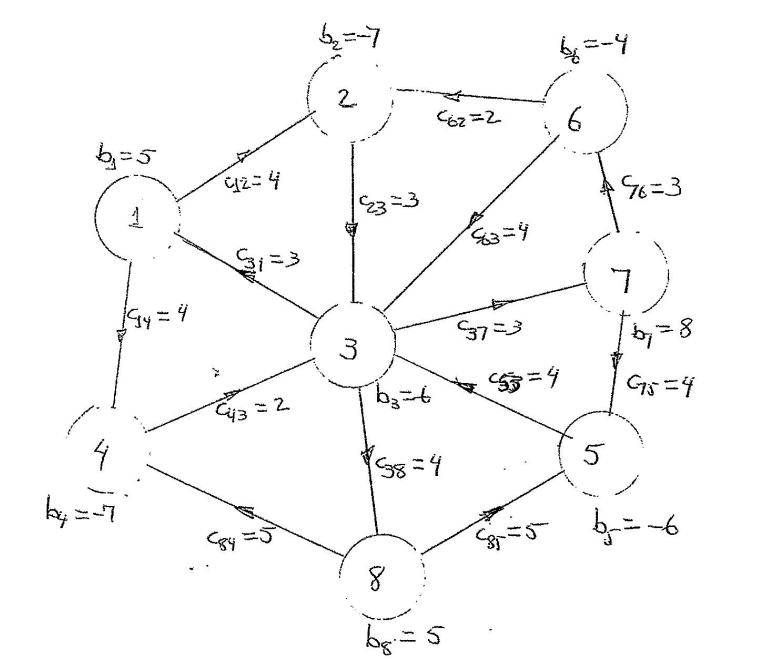
\includegraphics[scale=0.7]{images/q1-enunciado.png}
    \caption{Grafo orientado do problema de transbordo.}
\end{figure}

Para este problema de transbordo, foi gerado uma solução básica inicial (inviável) indicada na figura da página seguinte.
Observe que $x^{B}_{34}$ é uma variável artificial pois não há no grafo original o arco orientado (3, 4).
Na figura abaixo estão indicados os valores dos custos $d_{ij}^{B}$ das variáveis básicas para a fase 1.

\begin{figure}[H]
    \centering
    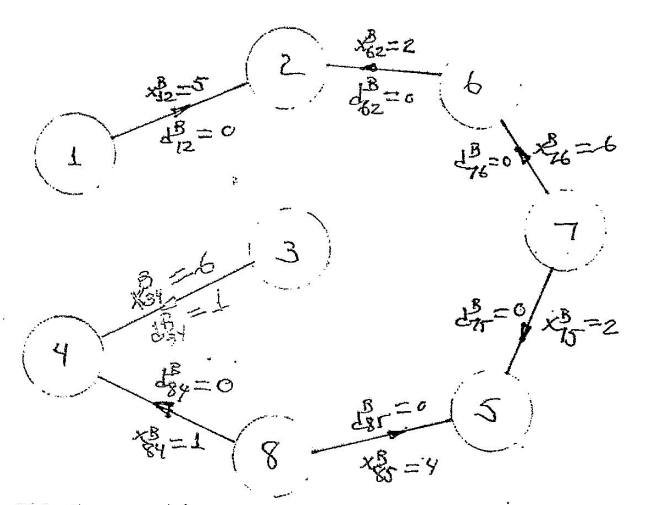
\includegraphics[scale=0.6]{images/q1-enunciado2.png}
    \caption{Solução básica inicial (inviável)}
\end{figure}


\subsection{item a)}

Ao fim da primeira iteração da fase 1, há um tríplice empate para a escolha da variável não básica atual que vai se tornar básica.
Opte por uma delas e vá até o fim da fase 2, para as outras duas, vá apenas até o fim da fase 1.


\subsubsection{Solução}

Começamos o exercício com a fase 1, na qual o objetivo é minimizar a soma das variáveis artificiais, que são variáveis de folga que foram adicionadas ao problema para possibilitar a resolução.
Neste caso, a única variável artificial é $x^{B}_{34}$, já que ela é a única que seu arco não existe no grafo original.

Partimos do grafo mostrado na figura abaixo, em que os arcos associados às variáveis não básicas estão representados com linhas tracejadas, enquanto as variáveis básicas recebem linhas contínuas.

\begin{figure}[H]
    \centering
    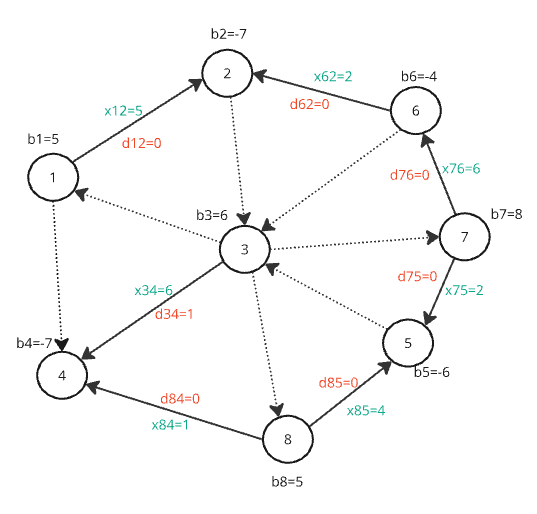
\includegraphics[scale=0.7]{images/grafo-res-1.png}
    \caption{Grafo mostrando a solução básica inicial (inviável) em linhas cheias e variáveis não básicas em linhas tracejadas.}
\end{figure}


Para as variáveis básicas, temos a propriedade de que $d_{ij}^{B} = \pi_{i} - \pi_{2}$.
Sabemos os valores de todos os $d_{ij}^{B}$, já que somente uma única variável ($x_{34}$) é artificial e, portanto, essa será o único caso em que $d_{ij}^{B} = 1$ (todos os outros casos serão $d_{ij}^{B} = 0$).
Dessa forma, fazemos:

\begin{align*}
    d_{12}^{B} = \pi_{1} - \pi_{2} &= 0 \\
    d_{62}^{B} = \pi_{6} - \pi_{2} &= 0 \\
    d_{76}^{B} = \pi_{7} - \pi_{6} &= 0 \\
    d_{75}^{B} = \pi_{7} - \pi_{5} &= 0 \\
    d_{85}^{B} = \pi_{8} - \pi_{5} &= 0 \\
    d_{84}^{B} = \pi_{8} - \pi_{4} &= 0 \\
    d_{34}^{B} = \pi_{3} - \pi_{4} &= 1 \\
\end{align*}

Como temos 7 equações para 8 variáveis, podemos arbitrar um valor de $\pi_{2} = 0$, por exemplo, e resolver o sistema linear acima para encontrar os valores de $\pi_{i}$.
Resolvendo, obtemos o seguinte resultado:

\begin{align*}
    \pi_{1} &= 0 \\
    \pi_{2} &= 0 \\
    \pi_{3} &= 1 \\
    \pi_{4} &= -1 \\
    \pi_{5} &= 0 \\
    \pi_{6} &= 0 \\
    \pi_{7} &= 0 \\
    \pi_{8} &= 0 \\
\end{align*}

Agora, para as variáveis não básicas, que são aquelas que representam os arcos que não estão incluídos na solução e, portanto, desenhados com linhas tracejadas na figura anterior, sabemos que $\overline{d}^{N}_{ij} = d^{N}_{ij} - \pi_{i} + \pi_{j}$.
Sendo assim, podemos fazer:

% TODO: cuidado, não vale se o dij for 1
\begin{align*}
    \overline{d}^{N}_{14} = \pi_{1} - \pi_{4} &=  0 \\
    \overline{d}^{N}_{31} = \pi_{3} - \pi_{1} &= -1 \\
    \overline{d}^{N}_{23} = \pi_{2} - \pi_{3} &=  1 \\
    \overline{d}^{N}_{63} = \pi_{6} - \pi_{3} &=  1 \\
    \overline{d}^{N}_{37} = \pi_{3} - \pi_{7} &= -1 \\
    \overline{d}^{N}_{53} = \pi_{5} - \pi_{3} &=  1 \\
    \overline{d}^{N}_{38} = \pi_{3} - \pi_{8} &= -1 \\
\end{align*}

Como existem 3 variáveis não básicas com $\overline{d}^{N}_{ij} \leq 0$, a solução atual não é ótima e portanto precisamos continuar com o método da fase 1.
De fato, agora podemos ver que há um tríplice empate para decidirmos qual variável não básica atual se tornará básica.
No caso, as variáveis $x^{N}_{31}$, $x^{N}_{37}$ e $x^{N}_{38}$ têm $\overline{d}^{N}_{ij} = -1$ e, portanto, são candidatas a se tornarem básicas.
Como solicitado pelo enunciado, vamos resolver o método da fase 1 para os 3 casos, além disso vamos escolher um dos 3 casos para resolver até o final da fase 2.


\subsubsection{Caso A: $x_{31}$ entra na base}

Aqui escolheremos a variável $x^{N}_{31}$ para entrar na base.
Devemos analisar qual das variáveis básicas atuais sairá da base.
Para isso, vamos analisar qual o valor máximo de $\theta$ que podemos atribuir para a variável $x^{B}_{31}$, de forma que outras variáveis básicas não sejam negativadas.
Para tanto, fazemos o balanço de massa para cada um dos nós já com a nova variável básica $x^{B}_{31}$, conforme segue:

\begin{align}
    \text{Nó 1:} & \quad b_{1} + x^{B}_{31} - x^{B}_{12} = 0 \\
    \text{Nó 2:} & \quad b_{2} + x^{B}_{12} + x^{B}_{62} = 0 \\
    \text{Nó 3:} & \quad b_{3} - x^{B}_{31} - x^{B}_{34} = 0 \\
    \text{Nó 4:} & \quad b_{4} + x^{B}_{84} + x^{B}_{34} = 0 \\
    \text{Nó 5:} & \quad b_{5} + x^{B}_{85} + x^{B}_{75} = 0 \\
    \text{Nó 6:} & \quad b_{7} + x^{B}_{76} - x^{B}_{62} = 0 \\
    \text{Nó 7:} & \quad b_{7} - x^{B}_{76} - x^{B}_{75} = 0 \\
    \text{Nó 8:} & \quad b_{8} - x^{B}_{84} - x^{B}_{85} = 0
\end{align}


Considerando que $x^{B}_{31} = \theta$ e simplificando as equações acima, temos:

\begin{align*}
    x^{B}_{31} &= \theta \\
    x^{B}_{34} &= 6 - \theta \\
    x^{B}_{84} &= 1 + \theta \\
    x^{B}_{85} &= 4 - \theta \\
    x^{B}_{75} &= 2 + \theta \\
    x^{B}_{76} &= 6 - \theta \\
    x^{B}_{62} &= 2 - \theta \\
    x^{B}_{12} &= 5 + \theta \\
\end{align*}

Podemos verificar que o máximo valor de $\theta$ será $\theta=2$, caso em que a variável $x^{B}_{62}$ se iguala a zero.
Sendo assim, escolhemos a variável $x^{B}_{62}$ para sair da base.

Temos que recalcular os valores das variáveis de decisão que vamos atribuir para cada arco básico.
Para tanto, basta igualar $\theta$ a $2$ e resolver o sistema linear mencionado logo acima.
O resultado será o grafo mostrado a seguir:

\begin{figure}[H]
    \centering
    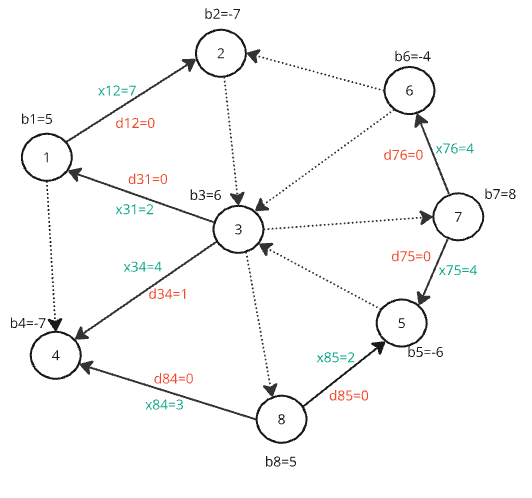
\includegraphics[scale=0.7]{images/grafo-res-2.png}
    \caption{Solução básica atual em linhas cheias e variáveis não básicas em linhas tracejadas.}
\end{figure}


Em seguida devemos verificar a otimalidade dessa solução.
De início já podemos imaginar que não é ótima ainda, visto que ainda resta uma variável artificial na base, mas precisamos testar.
Calculamos, então, para cada variável básica, a expressão dos multiplicadores:

\begin{align*}
    d_{12}^{B} = \pi_{1} - \pi_{2} &= 0 \\
    d_{31}^{B} = \pi_{3} - \pi_{1} &= 0 \\
    d_{76}^{B} = \pi_{7} - \pi_{6} &= 0 \\
    d_{75}^{B} = \pi_{7} - \pi_{5} &= 0 \\
    d_{85}^{B} = \pi_{8} - \pi_{5} &= 0 \\
    d_{84}^{B} = \pi_{8} - \pi_{4} &= 0 \\
    d_{34}^{B} = \pi_{3} - \pi_{4} &= 1 \\
\end{align*}

Se novamente arbitrarmos um valor de $\pi_{2} = 0$, podemos resolver o sistema linear acima para encontrar os valores de $\pi_{i}$, conforme demonstrado a seguir:

\begin{align*}
    \pi_{1} &= 0 \\
    \pi_{2} &= 0 \\
    \pi_{3} &= 0 \\
    \pi_{4} &= -1 \\
    \pi_{5} &= 1 \\
    \pi_{6} &= 1 \\
    \pi_{7} &= 1 \\
    \pi_{8} &= -1 \\
\end{align*}

Agora precisamos calcular os coeficientes das variáveis não básicas, os quais utilizam o valor dos multiplicadores calculados anteriormente.

\begin{align*}
    \overline{d}^{N}_{14} = d^{N}_{14} + \pi_{1} - \pi_{4} &=  1 \\
    \overline{d}^{N}_{23} = d^{N}_{23} + \pi_{2} - \pi_{3} &=  0 \\
    \overline{d}^{N}_{62} = d^{N}_{62} + \pi_{6} - \pi_{2} &=  1 \\
    \overline{d}^{N}_{63} = d^{N}_{63} + \pi_{6} - \pi_{3} &=  1 \\
    \overline{d}^{N}_{37} = d^{N}_{37} + \pi_{3} - \pi_{7} &= -1 \\
    \overline{d}^{N}_{53} = d^{N}_{53} + \pi_{5} - \pi_{3} &=  1 \\
    \overline{d}^{N}_{38} = d^{N}_{38} + \pi_{3} - \pi_{8} &=  1 \\
\end{align*}

Com existe uma variável não básica com $\overline{d}^{N}_{ij} \leq 0$, a solução atual não é ótima e, portanto, precisamos continuar com o método da fase 1.
Neste caso, a variável $x^{N}_{37}$ é a candidata a entrar na base, visto que tem $\overline{d}^{N}_{37} = -1$.
Precisamos, então, descobrir que sairá da base.
Para tanto, refazemos os procedimentos anteriores, começando pelo balanço de massa:

\begin{align}
    \text{Nó 1:} & \quad b_{1} + x^{B}_{31} - x^{B}_{12} = 0 \\
    \text{Nó 2:} & \quad b_{2} + x^{B}_{12} = 0 \\
    \text{Nó 3:} & \quad b_{3} - x^{B}_{31} - x^{B}_{34} - x^{B}_{37} = 0 \\
    \text{Nó 4:} & \quad b_{4} + x^{B}_{84} + x^{B}_{34} = 0 \\
    \text{Nó 5:} & \quad b_{5} + x^{B}_{85} + x^{B}_{75} = 0 \\
    \text{Nó 6:} & \quad b_{7} + x^{B}_{76} = 0 \\
    \text{Nó 7:} & \quad b_{7} - x^{B}_{76} - x^{B}_{75} + x^{B}_{37} = 0 \\
    \text{Nó 8:} & \quad b_{8} - x^{B}_{84} - x^{B}_{85} = 0
\end{align}

Considerando que $x^{B}_{37} = \theta$ e simplificando as equações acima, temos:

\begin{align*}
    x^{B}_{37} &= \theta \\
    x^{B}_{31} &= 2 \\
    x^{B}_{34} &= 4 - \theta \\
    x^{B}_{84} &= 3 + \theta \\
    x^{B}_{85} &= 2 - \theta \\
    x^{B}_{75} &= 4 + \theta \\
    x^{B}_{76} &= 4 \\
    x^{B}_{12} &= 7
\end{align*}

Neste caso observamos que o valor máximo de $\theta$ será $\theta=2$, caso em que a variável $x^{B}_{85}$ se iguala a zero.
Desse modo, a variável $x^{B}_{85}$ sairá da base e a variável $x^{N}_{37}$ entrará na base.
Precisamos recalcular os valores das variáveis de decisão e remontar o grafo da solução.
O resultado é mostrado logo abaixo:

\begin{figure}[H]
    \centering
    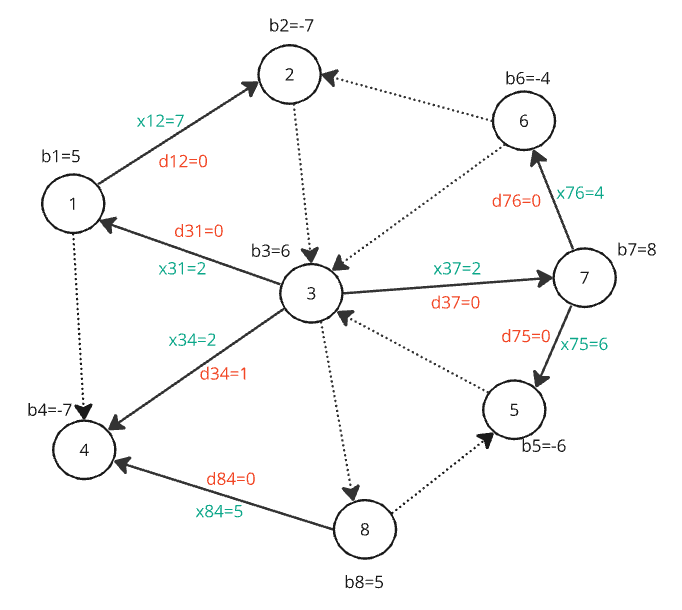
\includegraphics[scale=0.7]{images/grafo-res-3.png}
    \caption{Solução básica atual em linhas cheias e variáveis não básicas em linhas tracejadas.}
\end{figure}

Ainda possuímos uma variável artificial na base, então a solução atual não é ótima.
Vamos continuar.

Para as variáveis básicas, temos que:

\begin{align*}
    d_{12}^{B} = \pi_{1} - \pi_{2} &= 0 \\
    d_{31}^{B} = \pi_{3} - \pi_{1} &= 0 \\
    d_{76}^{B} = \pi_{7} - \pi_{6} &= 0 \\
    d_{75}^{B} = \pi_{7} - \pi_{5} &= 0 \\
    d_{37}^{B} = \pi_{3} - \pi_{7} &= 0 \\
    d_{84}^{B} = \pi_{8} - \pi_{4} &= 0 \\
    d_{34}^{B} = \pi_{3} - \pi_{4} &= 1 \\
\end{align*}

Supondo $\pi_{2} = 0$, podemos resolver o sistema linear acima para encontrar os valores de $\pi_{i}$, conforme segue:

\begin{align*}
    \pi_{1} &= 0 \\
    \pi_{2} &= 0 \\
    \pi_{3} &= 0 \\
    \pi_{4} &= -1 \\
    \pi_{5} &= 0 \\
    \pi_{6} &= 0 \\
    \pi_{7} &= 0 \\
    \pi_{8} &= -1 \\
\end{align*}

Já para as variáveis não básicas, temos que:

\begin{align*}
    \overline{d}^{N}_{14} = d^{N}_{14} + \pi_{1} - \pi_{4} &= 1 \\
    \overline{d}^{N}_{23} = d^{N}_{23} + \pi_{2} - \pi_{3} &= 0 \\
    \overline{d}^{N}_{62} = d^{N}_{62} + \pi_{6} - \pi_{2} &= 0 \\
    \overline{d}^{N}_{63} = d^{N}_{63} + \pi_{6} - \pi_{3} &= 0 \\
    \overline{d}^{N}_{53} = d^{N}_{53} + \pi_{5} - \pi_{3} &= 0 \\
    \overline{d}^{N}_{38} = d^{N}_{38} + \pi_{3} - \pi_{8} &= 1 \\
    \overline{d}^{N}_{85} = d^{N}_{85} + \pi_{8} - \pi_{5} &= -1 \\
\end{align*}

Como a variável $x^{N}_{85}$ tem $\overline{d}^{N}_{85} = -1$, ela é a candidata a entrar na base, apesar de ela ter acabado de sair da base.
Vamos manter as esperanças de que a variável de saída será outra, mas precisamos continuar com o método da fase 1.

Precisamos descobrir qual variável sairá da base.
Para tanto, vamos refazer o balanço de massa:

\begin{align}
    \text{Nó 1:} & \quad b_{1} + x^{B}_{31} - x^{B}_{12} = 0 \\
    \text{Nó 2:} & \quad b_{2} + x^{B}_{12} = 0 \\
    \text{Nó 3:} & \quad b_{3} - x^{B}_{31} - x^{B}_{34} - x^{B}_{37} = 0 \\
    \text{Nó 4:} & \quad b_{4} + x^{B}_{84} + x^{B}_{34} = 0 \\
    \text{Nó 5:} & \quad b_{5} + x^{B}_{75} + x^{B}_{85} = 0 \\
    \text{Nó 6:} & \quad b_{6} + x^{B}_{76} = 0 \\
    \text{Nó 7:} & \quad b_{7} - x^{B}_{76} - x^{B}_{75} + x^{B}_{37} = 0 \\
    \text{Nó 8:} & \quad b_{8} - x^{B}_{84} - x^{B}_{85} = 0
\end{align}

Considerando que $x^{B}_{85} = \theta$ e simplificando as equações acima, temos:

\begin{align*}
    x^{B}_{85} &= \theta \\
    x^{B}_{31} &= 2 \\
    x^{B}_{34} &= 2 + \theta \\
    x^{B}_{84} &= 5 - \theta \\
    x^{B}_{75} &= 6 - \theta \\
    x^{B}_{76} &= 4 \\
    x^{B}_{12} &= 7 \\
    x^{B}_{37} &= 2 - \theta \\
\end{align*}

Nesta etapa vemos que o valor limite de $\theta$ seria $\theta=2$, caso em que a variável $x^{B}_{34}$ se iguala a zero e, portanto, deveria sair da base.
Contudo, como acabamos de passar por uma troca entre $x^{B}_{37}$ e $x^{B}_{85}$, a variável $x^{B}_{34}$ não pode sair da base.
Dessa forma, a solução atual não é ótima mas não conseguimos mais melhorá-la com o método da fase 1.

\subsubsection{Caso B: $x_{37}$ entra na base}

Neste caso vamos considerar que a variável $x^{N}_{37}$ entra na base.
Precisamos descobrir qual variável sairá da base.



\subsubsection{Caso C: $x_{38}$ entra na base}

Neste caso vamos considerar que a variável $x^{N}_{38}$ entra na base.
Precisamos descobrir qual variável sairá da base.

\subsection{item b)}

O que aconteceria com a solução ótima do problema de transbordo, encontrada no item a), caso fosse alterada a orientação do arco (4, 3) e mantido o mesmo custo unitário de transporte?


\subsubsection{Solução}



\section{Questão 2}

Considere o problema de transbordo representado no grafo orientado abaixo.
Observe que há excesso de oferta nos nós da rede.
Conforme mencionado nas notas de aula, cria-se um centro consumidor fictício 8, com parâmetro $b_{8} = \sum_{i=1}^{7} b_{i}$ e arcos $(i, 8)$ ligando todo centro produtor $i$ ao centro consumidor fictício 8, com custos unitários de transporte nulos $c_{i8} = 0$.

\begin{figure}[H]
    \centering
    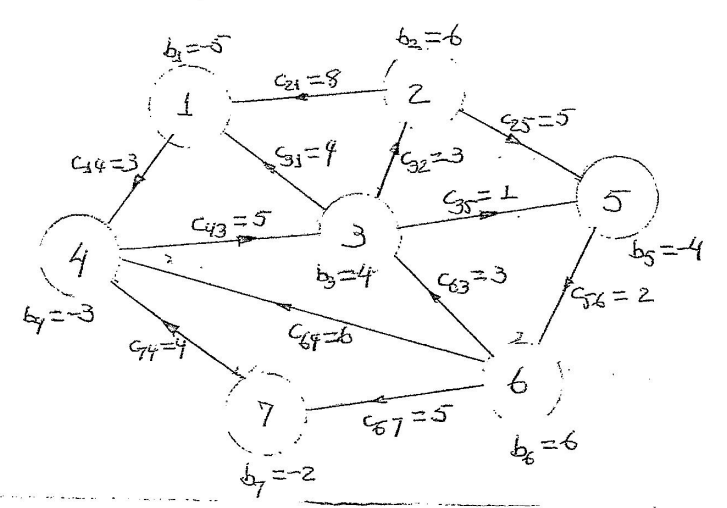
\includegraphics[scale=0.5]{images/q2-enunciado.png}
    \caption{Grafo do problema de transbordo 2}
\end{figure}


Para este problema de transbordo, foi gerada uma solução básica, com as seguintes variáveis básicas:
$x^{B}_{21} = 6$,
$x^{B}_{14} = 1$,
$x^{B}_{64} = 2$,
$x^{B}_{67} = 4$,
$x^{B}_{75} = 2$,
$x^{B}_{35} = 2$,
$x^{B}_{38} = 2$.

Observe que $x^{B}_{75}$ é uma variável artificial pois não existe no grafo orientado o arco (7, 5), e que $x^{B}_{38}$ é a oferta não utilizada do nó 3.

Determine uma solução ótima para o problema a partir da solução básica inicial inviável acima apresentada.


\subsection{Solução}

Vamos desenhar um grafo orientado representando o problema, mas dessa vez acrescentando o nó fictício 8 e os seus respectivos arcos que o ligam até os nós produtores.
Calcula-se a demanda fictícia do nó 8 de modo a alcançar o equilíbrio entre oferta e demanda.

\begin{figure}[H]
    \centering
    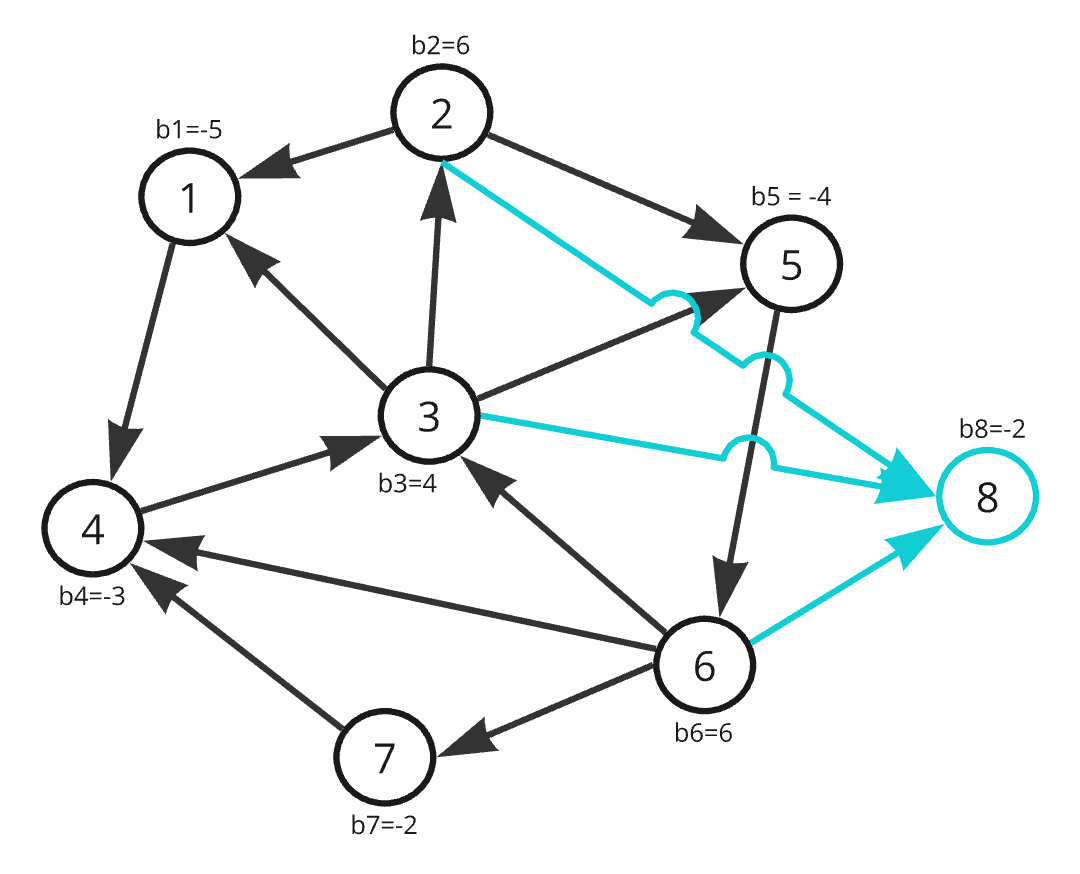
\includegraphics[scale=0.6]{images/q2-grafo-inicial.png}
    \caption{Grafo do problema de transbordo 2 com o nó fictício 8 e os arcos que o ligam aos nós produtores.}
\end{figure}


Vamos ter que usar o método das fases para resolver este problema, já que o enunciado aponta a existência de variáveis artificiais.
Através dos valores das variáveis básicas, vamos definir os valores de $d_{ij}^{B}$ associados ao grafo.

\begin{align*}
    d_{21} &= 0 \\
    d_{14} &= 0 \\
    d_{64} &= 0 \\
    d_{67} &= 0 \\
    d_{75} &= 1 \\
    d_{35} &= 0 \\
    d_{38} &= 0
\end{align*}

Podemos também separar o grafo entre variáveis básicas e não básicas, conforme mostrado na figura a seguir.

\begin{figure}[H]
    \centering
    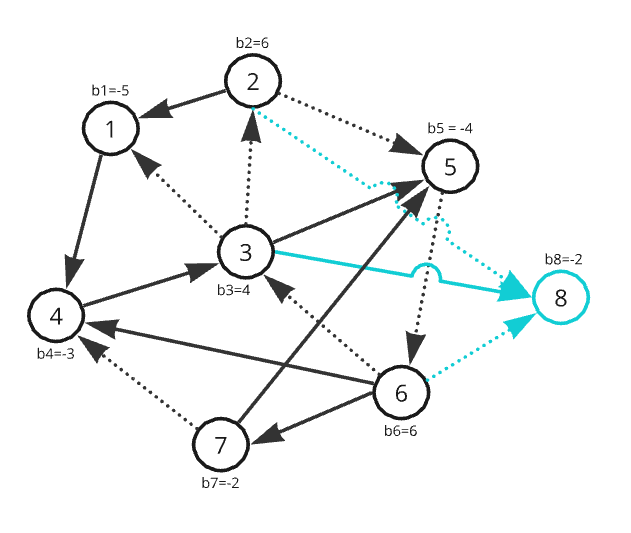
\includegraphics[scale=0.6]{images/q2-sol-inicial.png}
    \caption{Grafo do problema de transbordo 2 com variáveis básicas em linhas cheias e variáveis não básicas em linhas tracejadas.}
\end{figure}

Com isso já podemos calcular os multiplicadores:

\begin{align*}
    d_{21} &= \pi_{2} - \pi_{1} = 0 \\
    d_{14} &= \pi_{1} - \pi_{4} = 0 \\
    d_{64} &= \pi_{6} - \pi_{4} = 0 \\
    d_{67} &= \pi_{6} - \pi_{7} = 0 \\
    d_{75} &= \pi_{7} - \pi_{5} = 1 \\
    d_{35} &= \pi_{3} - \pi_{5} = 0 \\
    d_{38} &= \pi_{3} - \pi_{8} = 0
\end{align*}

Supondo $\pi_{2} = 2$, podemos obter:

\begin{align*}
    \pi_{1} &= 0 \\
    \pi_{2} &= 0 \\
    \pi_{3} &= -1 \\
    \pi_{4} &= 0 \\
    \pi_{5} &= -1 \\
    \pi_{6} &= 0 \\
    \pi_{7} &= 0 \\
    \pi_{8} &= -1 \\
\end{align*}

Para as variáveis não básicas, temos que:

\begin{align*}
    \overline{d}^{N}_{31} &= \pi_{3} - \pi_{1} = -1 \\
    \overline{d}^{N}_{32} &= \pi_{3} - \pi_{2} = -1 \\
    \overline{d}^{N}_{25} &= \pi_{2} - \pi_{5} = 1 \\
    \overline{d}^{N}_{56} &= \pi_{5} - \pi_{6} = -1 \\
    \overline{d}^{N}_{68} &= \pi_{6} - \pi_{8} = 1 \\
    \overline{d}^{N}_{74} &= \pi_{7} - \pi_{4} = 0 \\
    \overline{d}^{N}_{28} &= \pi_{2} - \pi_{8} = 1
\end{align*}

Notamos que há um empate entre três variáveis, então arbitrariamente escolhemos a variável $x^{N}_{32}$ para entrar na base.
Agora precisamos decidir qual das variáveis básicas sairá da base.
Precisamos definir o valor máximo de theta que a variável $x^{B}_{32}$ pode assumir sem que outras variáveis básicas sejam negativadas.

\begin{align}
    \text{Nó 1:} & \quad b_{1} + x_{21} - x_{14} = 0 \\
    \text{Nó 2:} & \quad b_{2} + x_{32} - x_{21} = 0 \\
    \text{Nó 3:} & \quad b_{3} - x_{32} - x_{35} + x_{43} - x_{38} = 0 \\
    \text{Nó 4:} & \quad b_{4} + x_{14} - x_{43} + x_{64} = 0 \\
    \text{Nó 5:} & \quad b_{5} + x_{35} - x_{75} = 0 \\
    \text{Nó 6:} & \quad b_{6} - x_{64} - x_{67} = 0 \\ 
    \text{Nó 7:} & \quad b_{7} - x_{75} + x_{67} = 0 \\
    \text{Nó 8:} & \quad b_{8} - x_{38} = 0
\end{align}

Sabendo que $x^{B}_{32} = \theta$, podemos simplificar as equações acima para:

\begin{align*}
    x^{B}_{32} &= \theta \\
    x^{B}_{21} &= 6 + \theta \\
    x^{B}_{14} &= 1 + \theta \\
    x^{B}_{38} &= 2 \\
\end{align*}

Os demais valores não podem ser isolados diretamente, pois o sistema é indeterminado.
Sendo assim, conclui-se que o modelo é ilimitado e não é possível resolvê-lo.
Muito provavelmente algum erro foi cometido no enunciado.

Utilizando o pacote OR-Tools, do Google, para resolver o sistema, utilizando os valores fornecidos no enunciado, chegamos à conclusão também de que o modelo é inviável (do inglês, \textit{infeasible}).

Utilizando o pacote OR-Tools, do Google, para resolver o sistema, utilizando os valores fornecidos no enunciado, chegamos à conclusão também de que o modelo é inviável (do inglês, \textit{infeasible}).

O código utilizado para tentar resolver o problema é mostrado a seguir, o qual está escrito em Python e utiliza o pacote OR-Tools.

\begin{lstlisting}[language=Python, caption=Exemplo de código Python utilizando OR-Tools]
import numpy as np

from ortools.graph.python import min_cost_flow


def main():
    """MinCostFlow simple interface example."""
    # Instantiate a SimpleMinCostFlow solver.
    smcf = min_cost_flow.SimpleMinCostFlow()

    # Define four parallel arrays: sources, destinations, capacities,
    # and unit costs between each pair. For instance, the arc from node 1
    # to node 4 has unit cost of 3.
    start_nodes = np.array([1, 2, 2, 2, 3, 3, 3, 3, 4, 5, 6, 6, 6, 6, 7])
    end_nodes = np.array([4, 1, 5, 8, 2, 1, 5, 8, 3, 6, 4, 7, 3, 8, 4])
    unit_costs = np.array([3, 8, 5, 0, 3, 4, 1, 0, 5, 2, 6, 5, 3, 0, 4])

    # define uma capacidade infinita
    capacities = np.array([1000]) * np.ones(len(start_nodes))

    # Define an array of supplies at each node.
    supplies = [
        -5,  # b1
        6,  # b2
        4,  # b3
        -3,  # b4
        -4,  # b5
        6,  # b6
        -2,  # b7
        -2,  # b8
    ]

    # Add arcs, capacities and costs in bulk using numpy.
    all_arcs = smcf.add_arcs_with_capacity_and_unit_cost(
        start_nodes, end_nodes, capacities, unit_costs
    )

    # Add supply for each nodes.
    smcf.set_nodes_supplies(np.arange(0, len(supplies)), supplies)

    # Find the min cost flow.
    status = smcf.solve()

    if status != smcf.OPTIMAL:
        print("There was an issue with the min cost flow input.")
        print(f"Status: {status}")
        exit(1)
    print(f"Minimum cost: {smcf.optimal_cost()}")
    print("")
    print(" Arc    Flow / Capacity Cost")
    solution_flows = smcf.flows(all_arcs)
    costs = solution_flows * unit_costs
    for arc, flow, cost in zip(all_arcs, solution_flows, costs):
        print(
            f"{smcf.tail(arc):1} -> {smcf.head(arc)}  {flow:3}  / {smcf.capacity(arc):3}       {cost}"
        )
\end{lstlisting}

Conforme comentado, a execução do código acima levou à conclusão de que o modelo é inviável.

\end{document}
